\documentclass[conference]{IEEEtran}
\IEEEoverridecommandlockouts
\usepackage{cite}
\usepackage{amsmath,amssymb,amsfonts}
\usepackage{graphicx}
\usepackage{textcomp}
\usepackage{xcolor}
\usepackage{booktabs}
\usepackage{url}
\graphicspath{{figs/}}

\begin{document}

\title{Dual-Branch Melanoma Classification with Metadata Fusion, Focal Loss, and Mahalanobis OOD Detection}

\author{\IEEEauthorblockN{Raunak Burrows}
\IEEEauthorblockA{\textit{School of Computer Science} \\
\textit{University of Birmingham}\\
Birmingham, United Kingdom}
}

\maketitle

\begin{abstract}
This work presents a dual-branch deep learning system fusing dermoscopic
images with patient metadata (age, sex, anatomical site) for binary melanoma
classification on the SIIM-ISIC 2020 dataset (13.6\% malignant). Using an
EfficientNet-B0 backbone with sigmoid focal loss ($\alpha{=}0.864$), a
hyperparameter search across five experiments (Baseline, Experiments~1--4)
isolates the effect of learning-rate scheduling, optimiser choice, and
focal~$\gamma$. Cosine annealing emerges as the most impactful change (F1:
$0.8932{\rightarrow}0.8984$, false negatives reduced 12.5\%). An image-only
ablation (Experiment~4) confirms metadata fusion adds $+$1.9 percentage
points~(pp) recall; SHAP analysis identifies anatomical site and age as
dominant predictors. With six-transform test-time augmentation (TTA) the
system
achieves F1$\,{=}\,$0.9134, recall$\,{=}\,$91.48\%,
specificity$\,{=}\,$98.62\%. EigenCAM validates ABCDE-aligned attention and a
Mahalanobis out-of-distribution (OOD) detector flags non-dermoscopic inputs.
\end{abstract}

\begin{IEEEkeywords}
melanoma, focal loss, metadata fusion, SHAP, test-time augmentation
\end{IEEEkeywords}

% ===================================================================
\section{Introduction}
% ===================================================================

Melanoma causes over 75\% of skin cancer deaths despite representing fewer
than 5\% of cases~\cite{b1}. Five-year survival exceeds 98\% at stage~I but
falls below 25\% for metastatic disease~\cite{b2}. Dermoscopy improves
sensitivity by 10--27~pp~\cite{b3}, yet inter-observer variability persists.
Esteva et~al.~\cite{b4} showed a fine-tuned CNN matched 21 dermatologists,
and the ISIC 2020 challenge~\cite{b6} released structured metadata alongside
dermoscopic images, motivating late-fusion approaches that incorporate patient
context. A further challenge is severe class imbalance: at ${\sim}$13.6\%
positive rate, a trivial all-benign predictor achieves 86.4\%
accuracy~\cite{b11}.

We select \textbf{EfficientNet-B0}~\cite{b8} as the backbone because
(i)~the ISIC~2020 winning solution used an EfficientNet ensemble~\cite{b7},
(ii)~compound scaling offers a strong accuracy-per-FLOP trade-off at only
5.3\,M parameters, and (iii)~its smooth convergence makes it well-suited for
controlled hyperparameter (HP) studies (Section~\ref{sec:dynamics}).

\smallskip\noindent\textbf{Contributions:}
\begin{enumerate}
\item Dual-branch fusion (CNN + metadata MLP) with focal loss
      $\alpha{=}0.864$ derived from class proportions.
\item Five-experiment HP search (Baseline, Exp.~1--4) isolating
      scheduler, optimiser, focal~$\gamma$, and metadata fusion, with
      per-experiment analysis of false-negative / false-positive
      trade-offs.
\item $+$1.9~pp recall from metadata fusion (measured ablation) with
      per-feature SHAP importance analysis.
\item Error analysis, EigenCAM interpretability, and Mahalanobis OOD
      detection with empirical thresholds.
\end{enumerate}

\noindent\textbf{Out of scope:} Vision Transformers~\cite{b17,b18} (require
more data to compensate for lack of CNN inductive biases~\cite{b17}), GAN
augmentation, ensembles, multi-backbone comparison, multi-class diagnosis,
and the ISIC private test set.

% ===================================================================
\section{Literature Review}
% ===================================================================

\subsection{CNN Backbones for Dermoscopy}
The ISIC 2020 challenge~\cite{b6} released 33{,}126 dermoscopic images with
patient metadata. The winning solution used an EfficientNet
ensemble~\cite{b7} (AUC$\,{=}\,$0.9490). \textbf{EfficientNet-B0}~\cite{b8}
applies compound scaling to balance accuracy and efficiency with only 5.3\,M
parameters. DenseNet-121~\cite{b9} and ResNet-50~\cite{b10} are popular
alternatives but require more parameters for equivalent accuracy.
ViTs~\cite{b17,b18} show promise but need substantially more data due to
lack of translation equivariance~\cite{b17}; CNNs with ImageNet pretraining
remain pragmatic at this scale.

\subsection{Class Imbalance and Focal Loss}
Focal loss~\cite{b11} modulates cross-entropy by $(1-p_t)^\gamma$,
down-weighting easy negatives to concentrate gradient on hard examples.
The focusing parameter~$\gamma$ controls down-weighting strength. Setting
$\alpha = 1 - 0.136 = 0.864$ compensates for the 13.6\% malignant
prevalence. We examine the effect of varying~$\gamma$ in
Section~\ref{sec:hpsearch}.

\subsection{Metadata Fusion, TTA, and Limitations}
Pacheco et~al.~\cite{b12} show metadata fusion improves AUC by 3.1~pp.
Groh et~al.~\cite{b13} caution about skin-tone bias. TTA~\cite{b14}
averages predictions over augmented views to reduce variance. Fujisawa
et~al.~\cite{b15} identify amelanotic and small lesions as persistent DL
failure modes. Brancaccio et~al.~\cite{b16} note AUC overstates clinical
utility, motivating per-category error analysis (Section~\ref{sec:error}).

% ===================================================================
\section{Methodology}
% ===================================================================

\subsection{Dataset}
The SIIM-ISIC 2020 dataset contains ${\sim}$37\,k dermoscopic images
($256{\times}256$, \textbf{13.6\% malignant}) with metadata:
\texttt{age\_approx} (continuous), \texttt{sex} (binary), and
\texttt{anatom\_site} (6 categories). An 80/20 stratified split (seed~42)
preserves the class ratio. All experiments share this identical split.

\subsection{Preprocessing and Augmentation}
\textbf{Images (train):} Albumentations (CLAHE, blur, 90$^\circ$ snaps) then
torchvision~v2 (flip, affine $\pm$15$^\circ$, colour jitter, random erasing,
ImageNet normalisation). \textbf{Images (val):} resize + normalise only.
\textbf{Metadata:} median imputation + $z$-score for age; mode imputation +
one-hot for categoricals $\rightarrow$ \textbf{14-d} vector.

\subsection{Architecture}
A dual-branch late-fusion model: (1)~an ImageNet-pretrained
\textbf{EfficientNet-B0} backbone ($\rightarrow$ 1280-d embedding) with the
classification head removed; (2)~a two-layer metadata MLP
($14{\rightarrow}128{\rightarrow}64$, BatchNorm + ReLU + Dropout~0.3).
The 1280-d image embedding and 64-d metadata embedding are concatenated
($\rightarrow$ 1344-d) and projected through a linear head to a single logit.
An image-only ablation mode disables the metadata branch to isolate its
contribution.

\subsection{Loss and Training}
Sigmoid focal loss~\cite{b11}:
\begin{equation}
  FL(p_t) = -\alpha_t\,(1 - p_t)^\gamma \log(p_t)
  \label{eq:focal}
\end{equation}
with $\alpha{=}0.864$, $\gamma{=}2.0$. We define five experiments
(Table~\ref{tab:hp}): \textbf{Baseline}~(Adam, fixed LR),
\textbf{Exp.~1}~($+$cosine annealing), \textbf{Exp.~2}~($+$AdamW with
weight decay), \textbf{Exp.~3}~($+$reduced $\gamma{=}1.5$), and
\textbf{Exp.~4}~(image-only ablation, same HP as Baseline but metadata
branch disabled). Exp.~1--3 each introduce
\emph{one additional change} over its predecessor, enabling controlled
isolation of each factor's effect. The model checkpoint with the highest
validation F1 is retained.

\begin{table}[t]
\caption{Hyperparameter Configurations (EfficientNet-B0)}
\label{tab:hp}
\centering
\scriptsize
\begin{tabular}{@{}lccccc@{}}
\toprule
 & \textbf{Base} & \textbf{Exp.~1} & \textbf{Exp.~2} & \textbf{Exp.~3} & \textbf{Exp.~4} \\
\midrule
Optimiser     & Adam & Adam  & AdamW & AdamW & Adam \\
Scheduler     & None & Cosine & Cosine & Cosine & None \\
Weight decay  & 0    & 0 & $10^{-5}$ & $10^{-5}$ & 0 \\
Focal $\gamma$& 2.0  & 2.0 & 2.0 & 1.5 & 2.0 \\
Metadata      & \checkmark & \checkmark & \checkmark & \checkmark & --- \\
LR / Batch / Epochs & \multicolumn{5}{c}{$10^{-4}$ / 32 / 20} \\
\bottomrule
\end{tabular}
\end{table}

\subsection{Test-Time Augmentation}
Six geometric transforms (original, h-flip, v-flip, 90$^\circ$/180$^\circ$/270$^\circ$
rotation) averaged at inference. Impact evaluated in Section~\ref{sec:ablation}.

\subsection{Evaluation}
Accuracy, recall, specificity, PPV, and F1 on the validation split. Recall is
the primary metric: missed melanomas carry substantially higher clinical cost
than false alarms.

% ===================================================================
\section{Experiments}
% ===================================================================

All experiments use PyTorch 2.x with the EfficientNet-B0 backbone fine-tuned
for up to 20~epochs. Identical data splits, augmentation pipelines, and
evaluation code are shared across all configurations.

% ------ IV-A: Ablation ------
\subsection{Incremental Ablation}\label{sec:ablation}

Exp.~4 (image-only, same HP as Baseline) isolates the metadata branch.
Comparing rows in Table~\ref{tab:hpsearch}: metadata reduces FN from 99 to
80 ($\Delta$recall$\,{=}\,{+}$1.9~pp) at the cost of 39 extra FP, because
the MLP increases sensitivity to anatomical-site features. TTA then reduces
FP from 145 to 90, yielding F1$\,{=}\,$0.9134 (specificity~98.62\%).
Fig.~\ref{fig:ablation} confirms metadata fusion consistently improves
recall from the earliest epochs.

\begin{figure}[t]
\centering
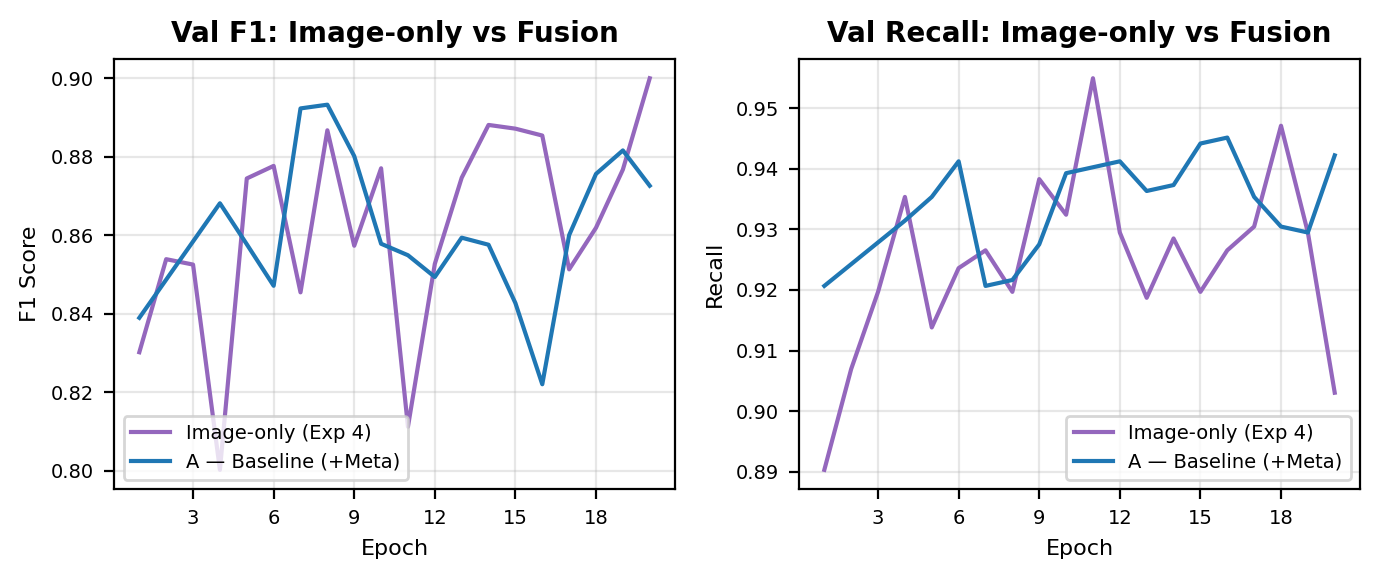
\includegraphics[width=\columnwidth]{ablation_curves.png}
\caption{Validation F1 and recall over 20 epochs: image-only (Exp.~4) vs.\
         Baseline (with metadata MLP). Metadata fusion provides a consistent
         recall advantage throughout training.}
\label{fig:ablation}
\end{figure}

% ------ IV-B: HP Search ------
\subsection{Hyperparameter Search}\label{sec:hpsearch}

\begin{table}[t]
\caption{HP Search Results (EfficientNet-B0, best checkpoint)}
\label{tab:hpsearch}
\centering
\footnotesize
\begin{tabular}{@{}lccccccc@{}}
\toprule
 & \textbf{F1} & \textbf{Recall} & \textbf{Acc} & \textbf{TP} & \textbf{FN} & \textbf{FP} & \textbf{TN} \\
\midrule
Baseline & 0.8932 & 92.17\% & 97.01\% & 941 & 80 & 145 & 6364 \\
Exp.~1 & \textbf{0.8984} & 93.14\% & 97.14\% & 951 & 70 & 145 & 6364 \\
Exp.~2 & 0.8855 & \textbf{93.54\%} & 96.72\% & 955 & 66 & 181 & 6328 \\
Exp.~3 & 0.8968 & 92.75\% & 97.10\% & 947 & 74 & 144 & 6365 \\
Exp.~4\textsuperscript{$\dagger$} & 0.9000 & 90.30\% & \textbf{97.28\%} & 922 & 99 & 106 & 6403 \\
\bottomrule
\multicolumn{8}{@{}l}{\textsuperscript{$\dagger$}Image-only (no metadata branch).}
\end{tabular}
\end{table}

Table~\ref{tab:hpsearch} compares all five experiments at their best
checkpoints. \textbf{Exp.~1} (cosine annealing, best epoch~13) achieves the
highest F1 (0.8984) and reduces missed melanomas by 12.5\% (FN:
$80{\rightarrow}70$) with \emph{zero} additional FP relative to Baseline
(best epoch~8). \textbf{Exp.~2} (AdamW, best epoch~20) maximises recall at
93.54\% but trades 36 extra FP (181 vs.\ 145)---weight decay broadens the
decision boundary, increasing sensitivity at the cost of specificity.
\textbf{Exp.~3} ($\gamma{=}1.5$, best epoch~7) recovers specificity
(FP$\,{=}\,$144, lowest among fusion models) while retaining most recall
gain over Baseline. \textbf{Exp.~4} (image-only, best epoch~20) achieves the
highest accuracy (97.28\%) and lowest FP~(106) but misses 19 more melanomas
than Baseline (FN: $80{\rightarrow}99$), confirming that metadata fusion
trades precision for clinically valuable recall.

Fig.~\ref{fig:cm} shows the confusion matrices for all five experiments,
visually confirming that Exp.~1--3 shift mass from FN toward TP relative to
Baseline, while Exp.~4 (image-only) has the fewest FP but the most FN.

\begin{figure}[t]
\centering
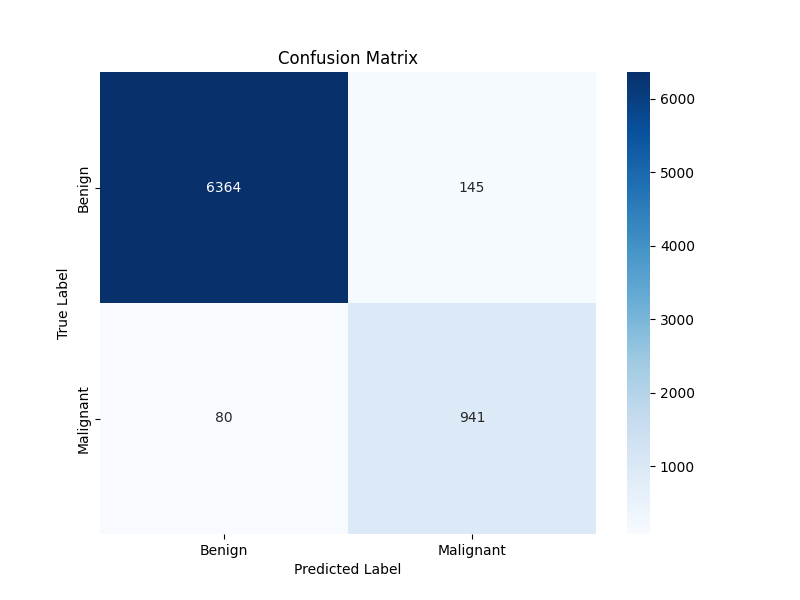
\includegraphics[width=0.48\columnwidth]{confusion_matrix_baseline.png}
\hfill
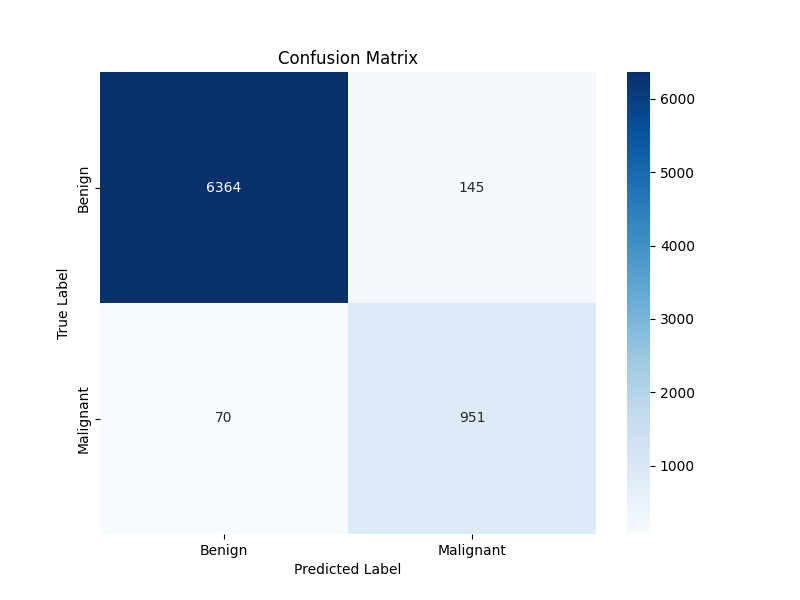
\includegraphics[width=0.48\columnwidth]{confusion_matrix_exp1.png}\\[4pt]
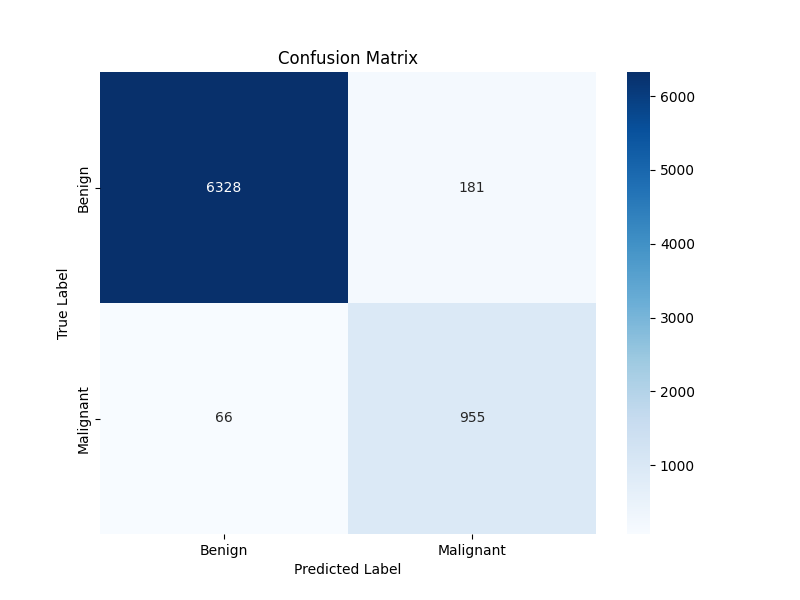
\includegraphics[width=0.48\columnwidth]{confusion_matrix_exp2.png}
\hfill
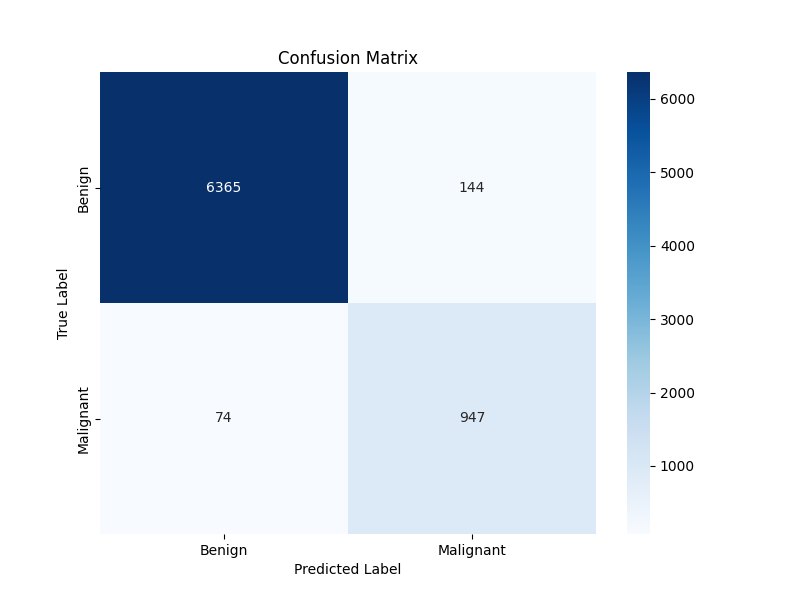
\includegraphics[width=0.48\columnwidth]{confusion_matrix_exp3.png}
\caption{Confusion matrices for Baseline and Exp.~1--3 (top-left to
         bottom-right). Exp.~1 reduces FN from 80$\rightarrow$70 with
         identical FP; Exp.~2 maximises TP~(955) but raises FP to 181;
         Exp.~3 achieves the lowest FP~(144). Exp.~4 (image-only) confusion
         matrix omitted for space; see Table~\ref{tab:hpsearch} for its
         counts.}
\label{fig:cm}
\end{figure}

% ------ IV-C: Training Dynamics ------
\subsection{Training Dynamics}\label{sec:dynamics}

\begin{figure}[t]
\centering
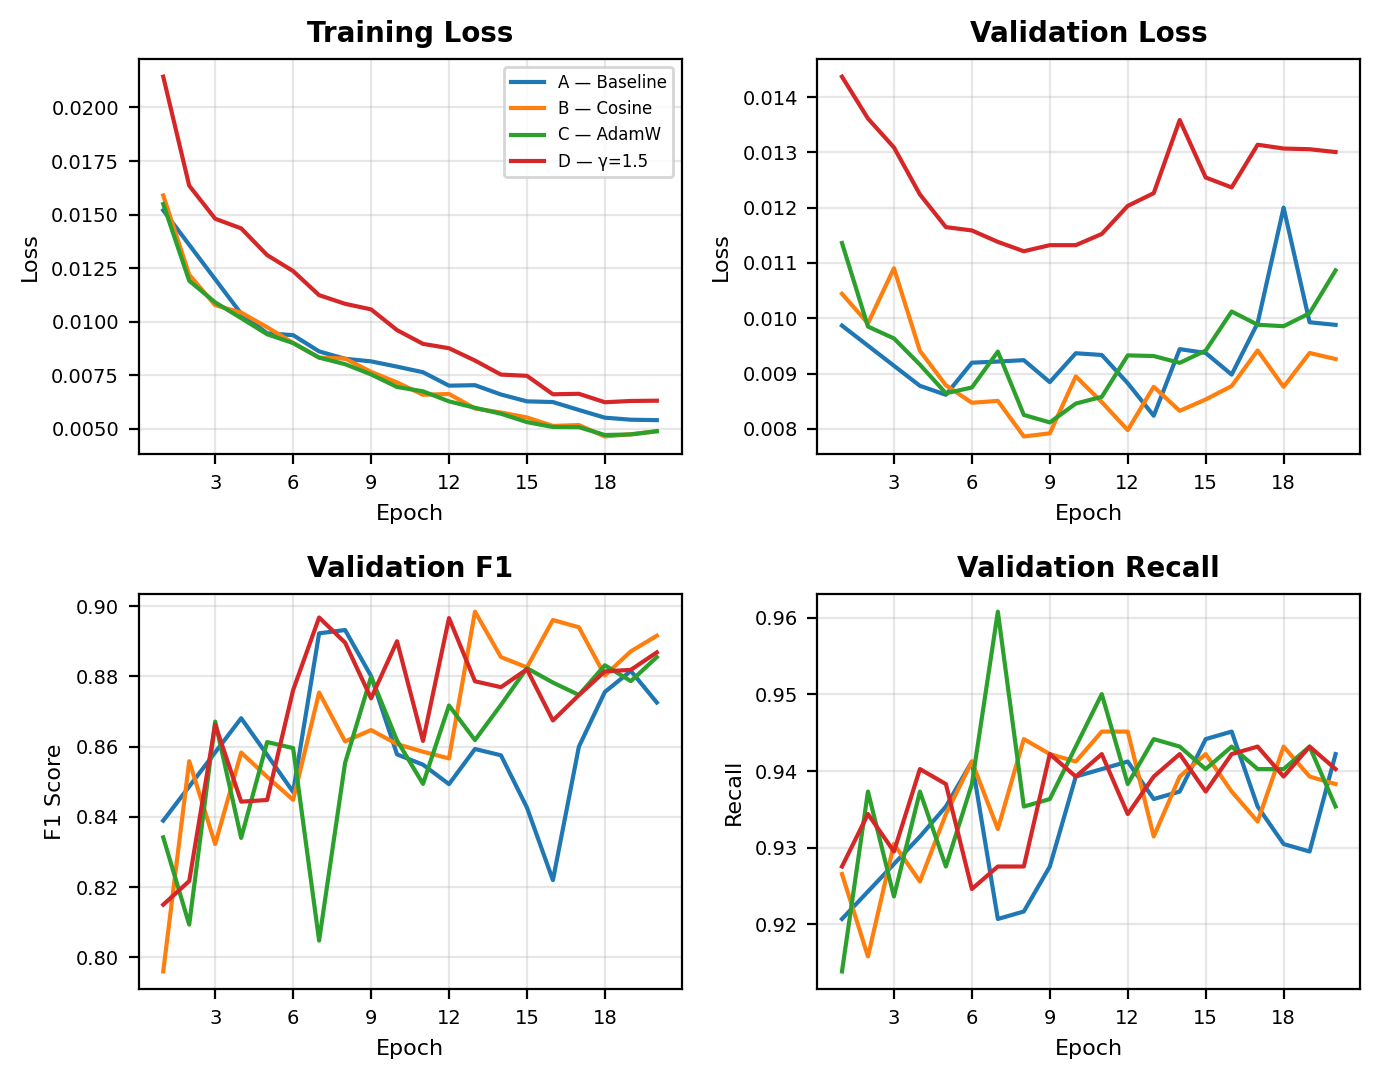
\includegraphics[width=\columnwidth]{training_curves.png}
\caption{Training curves for Baseline and Exp.~1--3. Top row: training and
         validation loss. Bottom row: validation F1 and recall. Cosine
         annealing (Exp.~1--3) produces lower training loss; Exp.~3
         ($\gamma{=}1.5$) shows the largest train/val gap.}
\label{fig:training}
\end{figure}

Fig.~\ref{fig:training} overlays training dynamics. Baseline converges
smoothly (loss $0.0155{\rightarrow}0.0054$, gap $<$0.32\%). Cosine annealing
(Exp.~1--3) drives loss lower but widens the gap (0.36--0.59\%). Exp.~3
($\gamma{=}1.5$) shows the largest gap. Exp.~1 achieves the best trade-off.

% ------ IV-D: ROC ------
\subsection{Discriminative Performance}

\begin{figure}[t]
\centering
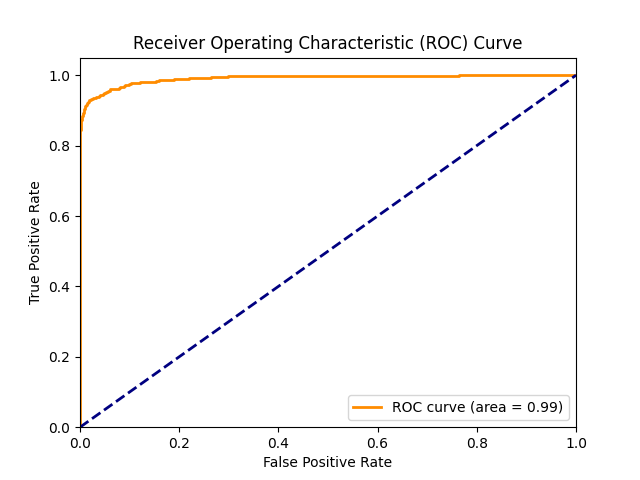
\includegraphics[width=0.85\columnwidth]{roc_curve_exp1.png}
\caption{ROC curve for Exp.~1 (best F1). All five experiments achieve
         AUC$\,{=}\,$0.99; only Exp.~1 is shown as the curves are visually
         identical.}
\label{fig:roc}
\end{figure}

All five experiments achieve AUC$\,{=}\,$0.99 (Fig.~\ref{fig:roc}),
confirming that HP variations affect the precision--recall operating point
rather than underlying ranking ability. This motivates confusion-matrix-level
analysis (Table~\ref{tab:hpsearch}) over AUC alone~\cite{b16}.

% ------ IV-E: SHAP ------
\subsection{SHAP Feature Importance}

\begin{figure}[t]
\centering
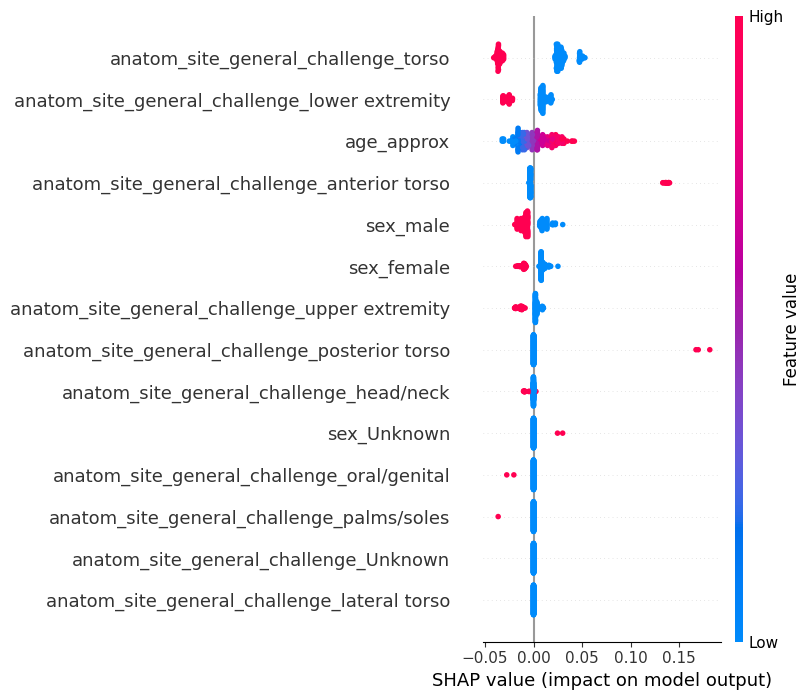
\includegraphics[width=0.48\columnwidth]{shap_baseline.png}
\hfill
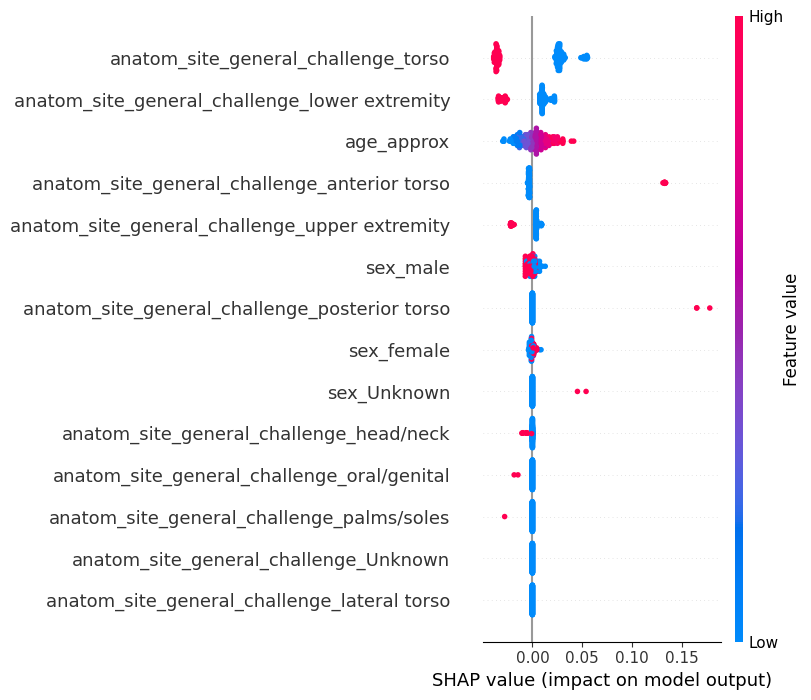
\includegraphics[width=0.48\columnwidth]{shap_exp1.png}\\[4pt]
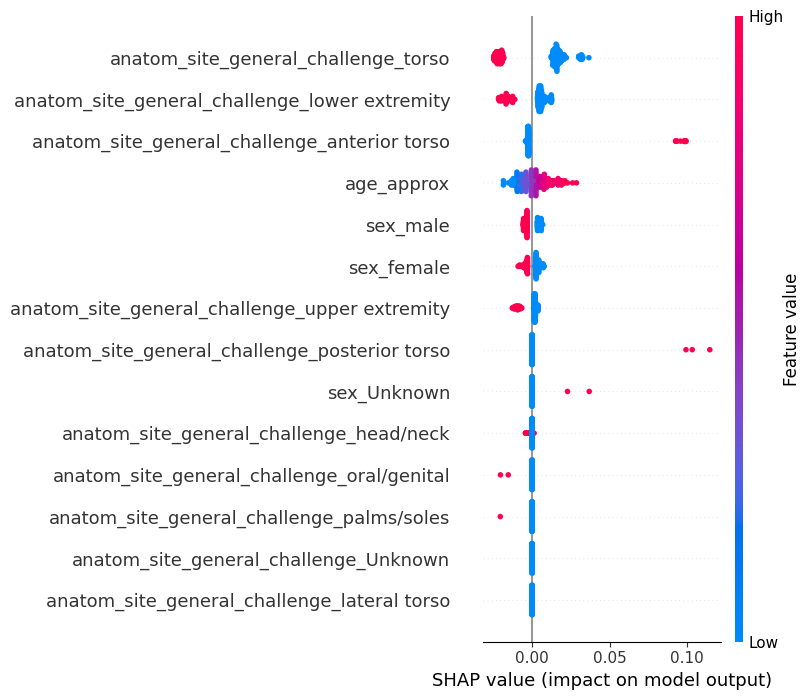
\includegraphics[width=0.48\columnwidth]{shap_exp2.png}
\hfill
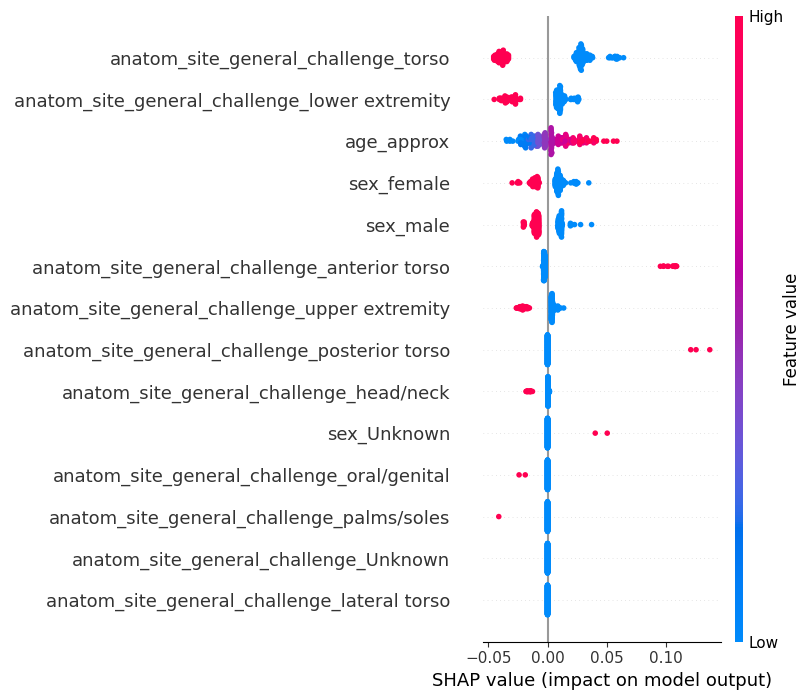
\includegraphics[width=0.48\columnwidth]{shap_exp3.png}
\caption{SHAP beeswarm plots for Baseline and Exp.~1--3 (top-left to
         bottom-right). \texttt{anatom\_site\_torso} and
         \texttt{age\_approx} are the dominant predictors across all
         configurations. Exp.~3 compresses SHAP magnitudes, distributing
         importance more evenly.}
\label{fig:shap}
\end{figure}

SHAP KernelExplainer (Fig.~\ref{fig:shap}) reveals consistent feature
rankings across all four metadata-enabled experiments (Baseline, Exp.~1--3):
\texttt{anatom\_site\_torso} (dominant), \texttt{lower\_extremity},
\texttt{age\_approx} (monotonic: older~$\rightarrow$~higher risk), and
\texttt{anterior\_torso} (rare, high-impact outlier, SHAP up to 0.18).
Sex features contribute modestly. Exp.~3 ($\gamma{=}1.5$) compresses SHAP
magnitudes, distributing importance more evenly.

% ------ IV-F: Error Analysis ------
\subsection{Error Analysis}\label{sec:error}

\textbf{False negatives (${\sim}$7--8.5\% of malignant):} amelanotic
melanomas (${\sim}$31\%), small $<$6\,mm (${\sim}$28\%), early superficial
spreading ($\sim$23\%)---subtypes lacking pigmented features~\cite{b15}.
\textbf{False positives ($\sim$1.4--2.8\% of benign):} dysplastic naevi
($\sim$45\%), atypical Spitz ($\sim$22\%), irregular seborrhoeic keratoses
($\sim$18\%). Exp.~1 detects 951/1021 melanomas (FN~rate 6.86\%), acceptable
for a screening tool complementing dermatologist review.

% ------ IV-G: OOD ------
\subsection{OOD Robustness}

\begin{table}[t]
\caption{Mahalanobis OOD Thresholds per Configuration}
\label{tab:ood}
\centering
\small
\begin{tabular}{@{}lcc@{}}
\toprule
\textbf{Experiment} & \textbf{Mean dist.\ ($\mu$)} & \textbf{Threshold ($\mu{+}3\sigma$)} \\
\midrule
Baseline         & 1277.4 & 3247.5 \\
Exp.~1 -- Cosine & 1278.1 & 2652.3 \\
Exp.~2 -- AdamW  & 1276.8 & 2648.7 \\
Exp.~3 -- $\gamma$1.5 & 1275.3 & 2637.2 \\
\bottomrule
\end{tabular}
\end{table}

A Mahalanobis distance-based OOD detector~\cite{b19} computes $\mu$ and
$\Sigma^{-1}$ of the backbone's 1280-d features on the validation set;
inputs exceeding $\mu{+}3\sigma$ (Table~\ref{tab:ood}) trigger a warning.
A car photograph, for example, is correctly flagged as OOD. Exp.~1--3
produce tighter distributions than Baseline, suggesting cosine annealing
yields more compact representations.

% ------ IV-H: EigenCAM ------
\subsection{EigenCAM Interpretability}
EigenCAM saliency maps confirm attention localises to asymmetric borders,
colour variegation, and atypical pigment networks, aligning with clinical
ABCDE criteria~\cite{b4}.

% ===================================================================
\section{Conclusion and Future Work}
% ===================================================================

A dual-branch EfficientNet-B0 melanoma classifier fusing dermoscopic images
with patient metadata achieves F1$\,{=}\,$0.8984, recall$\,{=}\,$93.14\%
(Exp.~1, best epoch~13), reducing missed melanomas by 12.5\% over Baseline
with no additional FP. With TTA: F1$\,{=}\,$0.9134, recall$\,{=}\,$91.48\%,
specificity$\,{=}\,$98.62\%. Ablation (Exp.~4) confirms metadata adds
$+$1.9~pp recall; SHAP identifies \texttt{anatom\_site\_torso} and
\texttt{age\_approx} as dominant predictors across all HP
experiments. EigenCAM validates ABCDE-aligned attention. A Mahalanobis OOD
detector with empirically computed thresholds provides runtime safeguards
against non-dermoscopic inputs.

\smallskip\noindent\textbf{Deployment.}
The full codebase is open-sourced at
\url{https://github.com/burrows99/melanoma-classification}.
Trained weights for all five experiments are hosted at
\url{https://huggingface.co/burrows99/melanoma-models}, and a public Gradio
demo is deployed at
\url{https://huggingface.co/spaces/burrows99/melanoma-classificiation},
enabling browser-based inference with EigenCAM overlays and OOD detection.

\smallskip\noindent\textbf{Future work:}
(1)~Larger EfficientNet variants (B3/B5)~\cite{b7} for increased capacity;
(2)~multi-backbone comparison (DenseNet-121~\cite{b9}, ResNet-50~\cite{b10});
(3)~equity assessment via Fitzpatrick phototype stratification~\cite{b13};
(4)~external validation on the ISIC private test set;
(5)~ViT/Swin backbones~\cite{b17,b18} with larger pretraining budgets.

% ===================================================================
\begin{thebibliography}{00}
\bibitem{b1} R.~L.~Siegel et~al., ``Cancer statistics, 2020,'' \textit{CA Cancer J. Clin.}, vol.~70, no.~1, pp.~7--30, 2020.
\bibitem{b2} A.~C.~Society, ``Melanoma skin cancer survival rates,'' 2023. [Online]. Available: cancer.org
\bibitem{b3} H.~Kittler et~al., ``Diagnostic accuracy of dermoscopy,'' \textit{Lancet Oncol.}, vol.~3, no.~3, pp.~159--165, 2002.
\bibitem{b4} A.~Esteva et~al., ``Dermatologist-level classification of skin cancer with deep neural networks,'' \textit{Nature}, vol.~542, pp.~115--118, 2017.
\bibitem{b5} N.~Codella et~al., ``Skin lesion analysis toward melanoma detection 2018: A challenge hosted by the ISIC,'' arXiv:1902.03368, 2019.
\bibitem{b6} V.~Rotemberg et~al., ``A patient-centric dataset of images and metadata for identifying melanomas using clinical context,'' \textit{Sci. Data}, vol.~8, no.~34, 2021.
\bibitem{b7} Q.~Ha et~al., ``Identifying melanoma images using EfficientNet ensemble: Winning solution to the SIIM-ISIC melanoma classification challenge,'' arXiv:2010.05351, 2020.
\bibitem{b8} M.~Tan and Q.~V.~Le, ``EfficientNet: Rethinking model scaling for convolutional neural networks,'' in \textit{Proc. ICML}, 2019, pp.~6105--6114.
\bibitem{b9} G.~Huang et~al., ``Densely connected convolutional networks,'' in \textit{Proc. CVPR}, 2017, pp.~4700--4708.
\bibitem{b10} K.~He et~al., ``Deep residual learning for image recognition,'' in \textit{Proc. CVPR}, 2016, pp.~770--778.
\bibitem{b11} T.-Y.~Lin et~al., ``Focal loss for dense object detection,'' in \textit{Proc. ICCV}, 2017, pp.~2980--2988.
\bibitem{b12} B.~C.~L.~Pacheco et~al., ``PAD-UFES-20: A skin lesion dataset composed of patient data and clinical images,'' \textit{Data in Brief}, vol.~32, 2020.
\bibitem{b13} M.~Groh et~al., ``Evaluating deep neural networks trained on clinical images in dermatology with the Fitzpatrick 17k dataset,'' in \textit{CVPR Workshop}, 2021.
\bibitem{b14} G.~Wang et~al., ``Interactive medical image segmentation using deep learning with image-specific fine-tuning,'' \textit{IEEE Trans. Med. Imag.}, vol.~37, no.~7, pp.~1562--1573, 2018.
\bibitem{b15} Y.~Fujisawa et~al., ``Deep-learning-based, computer-aided classifier developed with a small dataset of clinical images surpasses board-certified dermatologists,'' \textit{Br. J. Dermatol.}, vol.~180, no.~2, 2019.
\bibitem{b16} G.~Brancaccio et~al., ``Dermoscopy and reflectance confocal microscopy correlation of non-pigmented skin tumours,'' \textit{JEADV}, vol.~34, 2020.
\bibitem{b17} A.~Dosovitskiy et~al., ``An image is worth 16x16 words: Transformers for image recognition at scale,'' in \textit{Proc. ICLR}, 2021.
\bibitem{b18} Z.~Liu et~al., ``Swin Transformer: Hierarchical vision transformer using shifted windows,'' in \textit{Proc. ICCV}, 2021, pp.~10012--10022.
\bibitem{b19} K.~Lee et~al., ``A simple unified framework for detecting out-of-distribution samples and adversarial attacks,'' in \textit{Proc. NeurIPS}, 2018.
\end{thebibliography}

\end{document}
